% vim: set tw=78 sts=2 sw=2 ts=8 aw et ai:
\documentclass{workshop}

% Comentează liniile de mai jos în cazul în care nu există cod de inclus.
\usepackage{code/highlight}
\usepackage{color}        % dacă e folosit highlight
\usepackage{alltt}        % dacă e folosit highlight

\title[Sesssion 1]{Session 1}
\subtitle{Getting started with the Linux Kernel}
\author{Daniel Băluță, Irina Preșa}
\date{02 July 2012}

\begin{document}

% Arătăm numărul frame-ului
\setbeamertemplate{footline}[frame number]

\frame{\titlepage}

% NB: Secțiunile nu sunt marcate vizual, ci doar apar în cuprins
\section{Introduction}

\begin{frame}{Introduction}
//TODO Daniel
\end{frame}

\section{Source Code Browsing}

\begin{frame}{Source Code Browsing}
\end{frame}

\section{Booting and Initialization}
\subsection{Intro: Controllers and Hardware}
\begin{frame}{Intro: Controllers and Hardware}
     \begin{figure}
         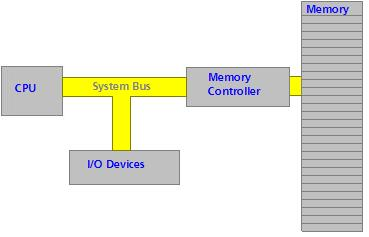
\includegraphics[scale=0.9]{img/bus.jpg}
      \end{figure}
\end{frame}

\begin{frame}{Intro: Controllers and Hardware}
\textbf{Real Mode}\\
\begin{itemize}
  \item CPU puts physical address on the bus.
  \item the memory controller recognizes it.
\end{itemize}

\textbf{Protected Mode}\\
\begin{itemize}
  \item CPU puts virtual address on the bus
  \item MMU translates it into a physical address
  \item memory protection
  \begin{itemize}
    \item 4 Operating Modes: Ring 0, Ring 1, Ring 2, Ring 3
  \end{itemize}
  \item hardware support for virtual memory
  \item can address more memory
\end{itemize}
\end{frame}

\begin{frame}{Intro: Controllers and Hardware}
\textbf{I/O Ports}\\
\begin{itemize}
  \item device controller listens on its ports.
  \item CPU puts port on the bus and sets the I/O access line.
  \item the controller of the associated device recognizes it.
  \item the memory controller will ignore the address.
  \item CPU offers IN/OUT instructions.
  \item ex: Intel interrupt controller.
\end{itemize}

\textbf{Memory Mapped I/O}\\
\begin{itemize}
  \item device controller mapped into memory.
  \item CPU puts address on the bus.
  \item the memory controller recognizes it.
  \item ex: ARM interrupt controller.
\end{itemize}
\end{frame}

\subsection{Before Kernel ...}
\begin{frame}{Before Kernel ...}
      \begin{figure}
         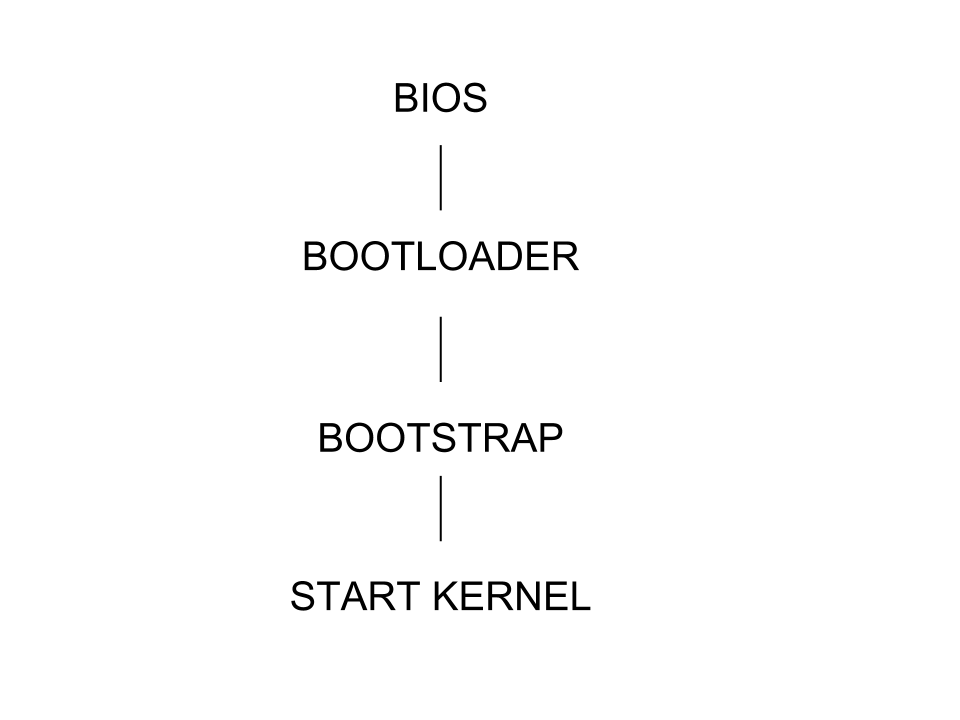
\includegraphics[scale=0.3]{img/boot.png}
      \end{figure}
\end{frame}

\begin{frame}{BIOS}
\end{frame}

\begin{frame}{Bootloader}
\end{frame}

\begin{frame}{Bootstrap}
\end{frame}

\begin{frame}{Extra: U-Boot}
      \begin{figure}
         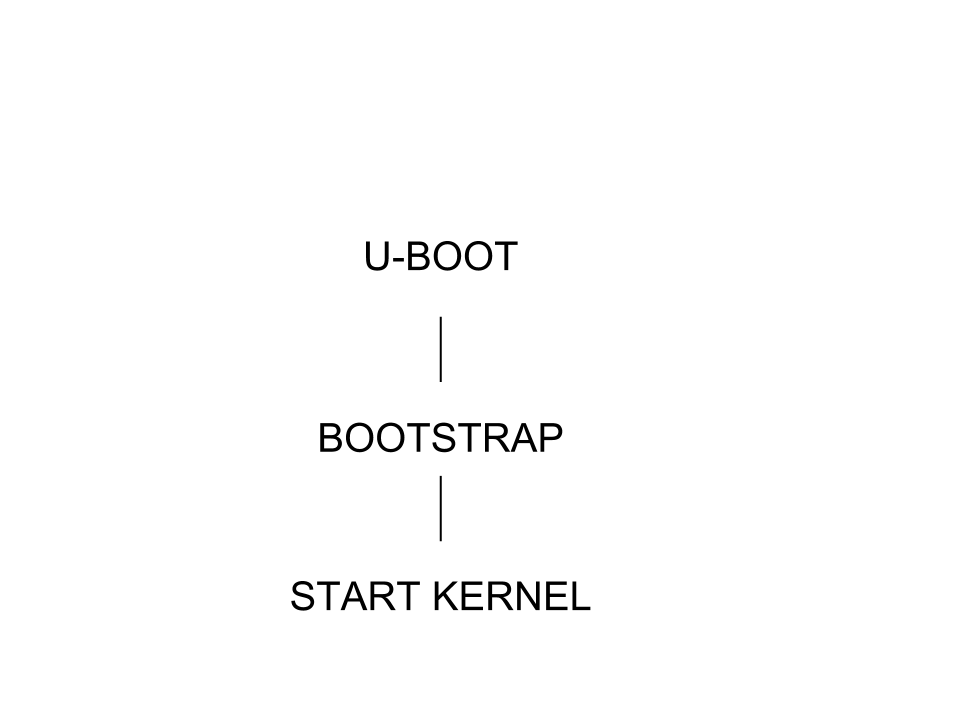
\includegraphics[scale=0.3]{img/u-boot.png}
      \end{figure}
\end{frame}

\begin{frame}{Extra: U-Boot}
% tfpt, fatload, burn and manage flash, etc
\end{frame}

\begin{frame}{Extra: Boot Embedded Device}
  \begin{columns}
    \begin{column}[l]{0.45\textwidth}
      \begin{figure}
         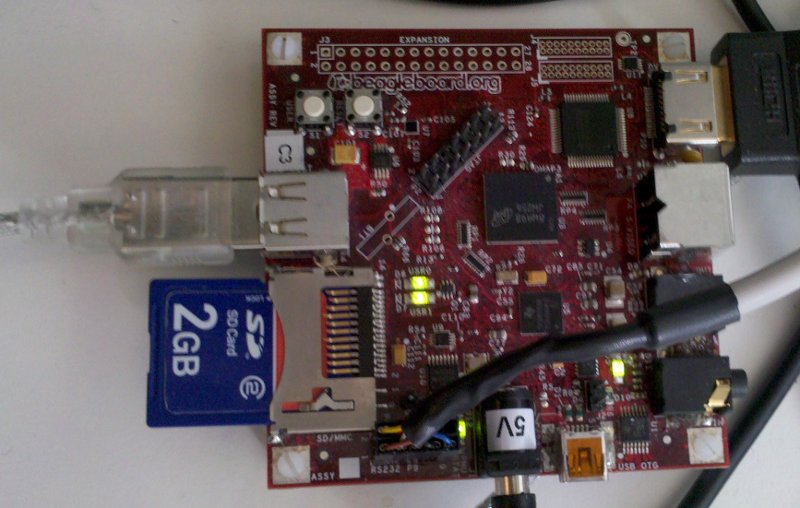
\includegraphics[scale=0.17]{img/beagle.jpg}
      \end{figure}
    \end{column}
    \begin{column}[l]{0.45\textwidth}
      \begin{figure}
         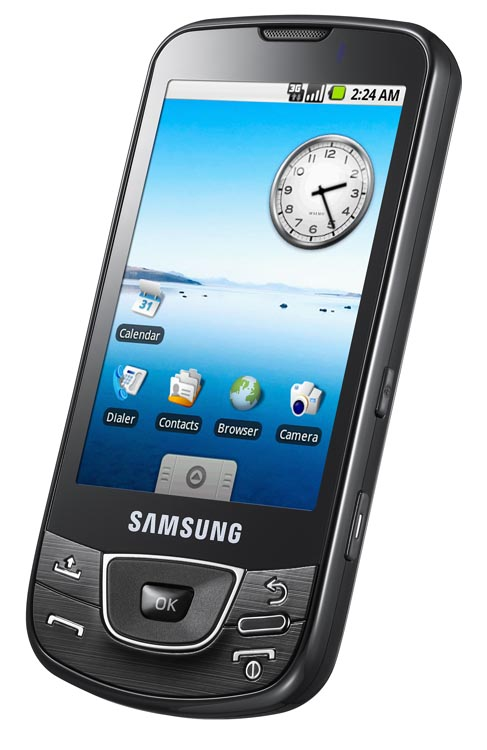
\includegraphics[scale=0.65]{img/phone.jpg}
      \end{figure}
    \end{column}
  \end{columns}
\end{frame}

\begin{frame}{Extra: Case Study}
  \begin{columns}
    \pause
    \begin{column}[l]{0.45\textwidth}
      \begin{figure}
         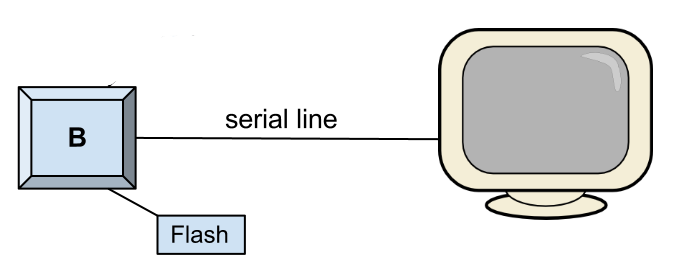
\includegraphics[scale=0.17]{img/flash.png}
      \end{figure}
      \begin{center}
        \tiny{- burn u-boot and kernel images on the flash.}
      \end{center}
    \end{column}
    \pause
    \begin{column}[l]{0.45\textwidth}
      \begin{figure}
         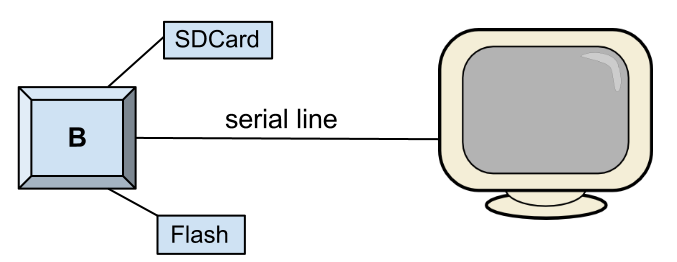
\includegraphics[scale=0.17]{img/sdcard.png}
      \end{figure}
      \begin{center}
        \tiny{- fatload mmc 0 8000 image.bin}
      \end{center}
    \end{column}
  \end{columns}
     \pause
     \begin{figure}
         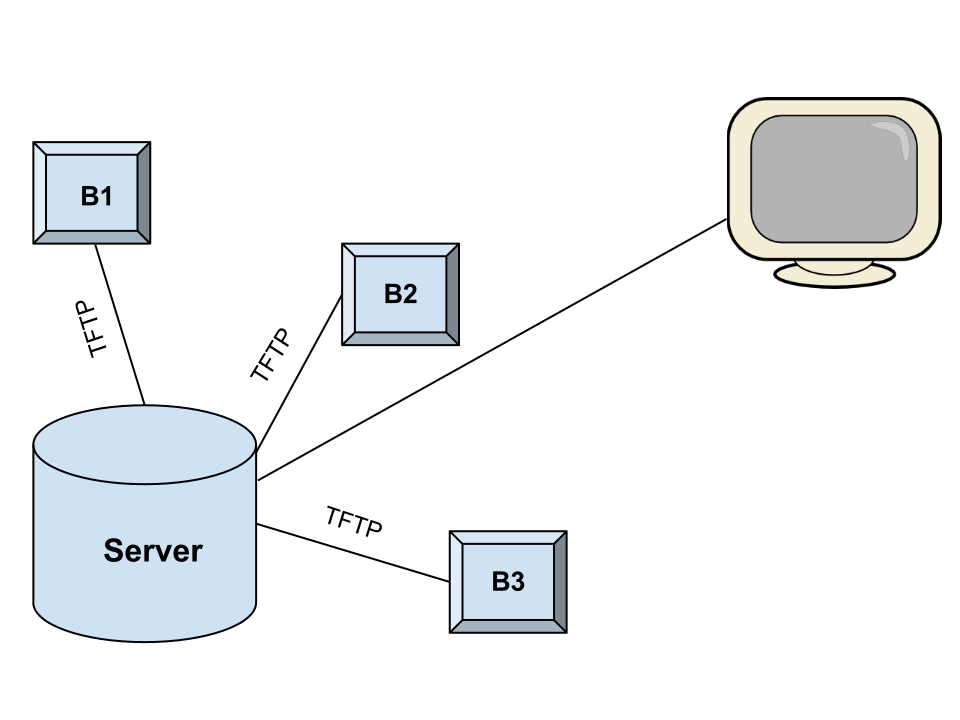
\includegraphics[scale=0.17]{img/complex.png}
      \end{figure}
      \begin{center}
      \tiny{- tftp 8000 image.bin}
      \end{center}
\end{frame}


\subsection{Startup Kernel ...}

\begin{frame}{Startup Kernel}

\textbf{Entry point...}\\
\begin{itemize}
\item startup\_32
\begin{itemize}
\item page tables
\item enable mmu
\end{itemize}
\end{itemize}

\textbf{Initialize...}\\
\begin{itemize}
\item start\_kernel
\begin{itemize}
\item trap\_init
\item mm\_init
\item init\_IRQ
\item sched\_init
\item time\_init
\item console\_init
\item smp\_init
\end{itemize}
\end{itemize}

\textbf{And.. UP!}\\
\begin{itemize}
\item rest\_init
\begin{itemize}
\item kernel\_thread
\item cpu\_idle
\end{itemize}
\end{itemize}
\end{frame}

\begin{frame}[fragile]{Cod verbatim}
  \pause
  \footnotesize
  \begin{verbatim}
brw-rw----  1 root disk      8,   0 Oct  2 21:53 sda
brw-rw----  1 root disk      8,   1 Oct  2 21:53 sda1
brw-rw----  1 root disk      8,  10 Oct  2 18:53 sda10
brw-rw----  1 root disk      8,  11 Oct  2 21:53 sda11
crw-rw----  1 root root      4,   0 Oct  2 21:53 tty0
crw-rw----  1 root root      4,  10 Oct  2 21:53 tty10
crw-rw----  1 root root      4,  11 Oct  2 21:53 tty11
crw-rw----  1 root root      4,  12 Oct  2 21:53 tty12
  \end{verbatim}
\end{frame}


\section{Keywords}

\begin{frame}{Keywords}
  \begin{columns}
    \begin{column}[l]{0.5\textwidth}
      \begin{itemize}
        \item cscope, ctags, lxr
        \item real vs protected mode
        \item ports vs memory mapped I/O
        \item 
        \item 
        \item 
        \item 
        \item 
      \end{itemize}
    \end{column}
    \begin{column}[l]{0.5\textwidth}
      \begin{itemize}
        \item 
        \item 
        \item 
        \item 
        \item 
        \item 
        \item 
        \item 
      \end{itemize}
    \end{column}
  \end{columns}
\end{frame}

\begin{frame}{Resources}
  \begin{itemize}
    \item \url{http://www.brokenthorn.com/Resources/OSDev7.html}
  \end{itemize}
\end{frame}

\section{Questions}

\end{document}
